% \documentclass[handout]{beamer}
\documentclass{beamer}
\usepackage[ruled,linesnumbered]{algorithm2e}
\usepackage{calc}  
%\usepackage{enumitem} 
\definecolor{vuborange}{rgb}{1.0,0.40,0.0}
\usetheme{Boadilla}
\title{Efficiently Explaining CSPs with Unsatisfiable Subset Optimization}

\institute[shortinst]
{\inst{1} Vrije Universiteit Brussel, Belgium \\ % Your institution for the title page
\inst{2} KULeuven, Belgium \\ % Your institution for the title page
\href{mailto:emilio.gamba@vub.be}{\underline{emilio.gamba@vub.be}}, \href{mailto:bart.bogaerts@vub.be}{bart.bogaerts@vub.be}, \href{mailto:tias.guns@kuleuven.be}{tias.guns@kuleuven.be} % Your email address
}
\date{IJCAI 2021}

\author{\underline{Emilio Gamba}\inst{1} \and  Bart Bogaerts\inst{1} \and   Tias Guns\inst{1,2}}

\newcommand\m[1]{\ensuremath{#1}\xspace}
\newcommand\allconstraints{\m{T_P}}
\newcommand\formula{\ensuremath{\m{F} }\xspace}
\newcommand\formulac{\ensuremath{\m{C} }\xspace}

\newcommand{\phantomgraphics}[2][]{%
  \leavevmode\phantom{\includegraphics[#1]{#2}}%
}


\makeatletter
\setbeamertemplate{footline}
{
  \leavevmode%
  \hbox{%
  \begin{beamercolorbox}[wd=.2\paperwidth,ht=2.25ex,dp=1ex,center]{author in head/foot}%
    \usebeamerfont{author in head/foot}Emilio Gamba (VUB)
  \end{beamercolorbox}%
  \begin{beamercolorbox}[wd=.6\paperwidth,ht=2.25ex,dp=1ex,center]{title in head/foot}%
    \usebeamerfont{title in head/foot}Efficiently Explaining CSPs with Unsatisfiable Subset Optimization
  \end{beamercolorbox}%
  \begin{beamercolorbox}[wd=.2\paperwidth,ht=2.25ex,dp=1ex,right]{date in head/foot}%
    \usebeamerfont{date in head/foot}August 2021\hspace*{1em}
    \insertframenumber{} / \inserttotalframenumber\hspace*{2ex} 
  \end{beamercolorbox}}%
  \vskip0pt%
}
\makeatother

\begin{document}

\begin{frame}
    \maketitle
    \vspace{-2.5cm}
\end{frame}


\begin{frame}
	\frametitle{Outline}
	\begin{enumerate}
		\item Motivation
		\begin{itemize}
			\item Explanations for CSPs
			\item Generating an explanation sequence for CSPs
		\end{itemize}
		\item Contributions and Applicability
		\begin{enumerate}
			\item Optimality
			\item Constrainedness
			\item Incrementality
		\end{enumerate}
	\item Results
	\item Conclusion
	
	\item Ideas for future work
	\end{enumerate}
\end{frame}

\begin{frame}{Motivation}
	\framesubtitle{Logic Grid Puzzles}
	\begin{figure}
		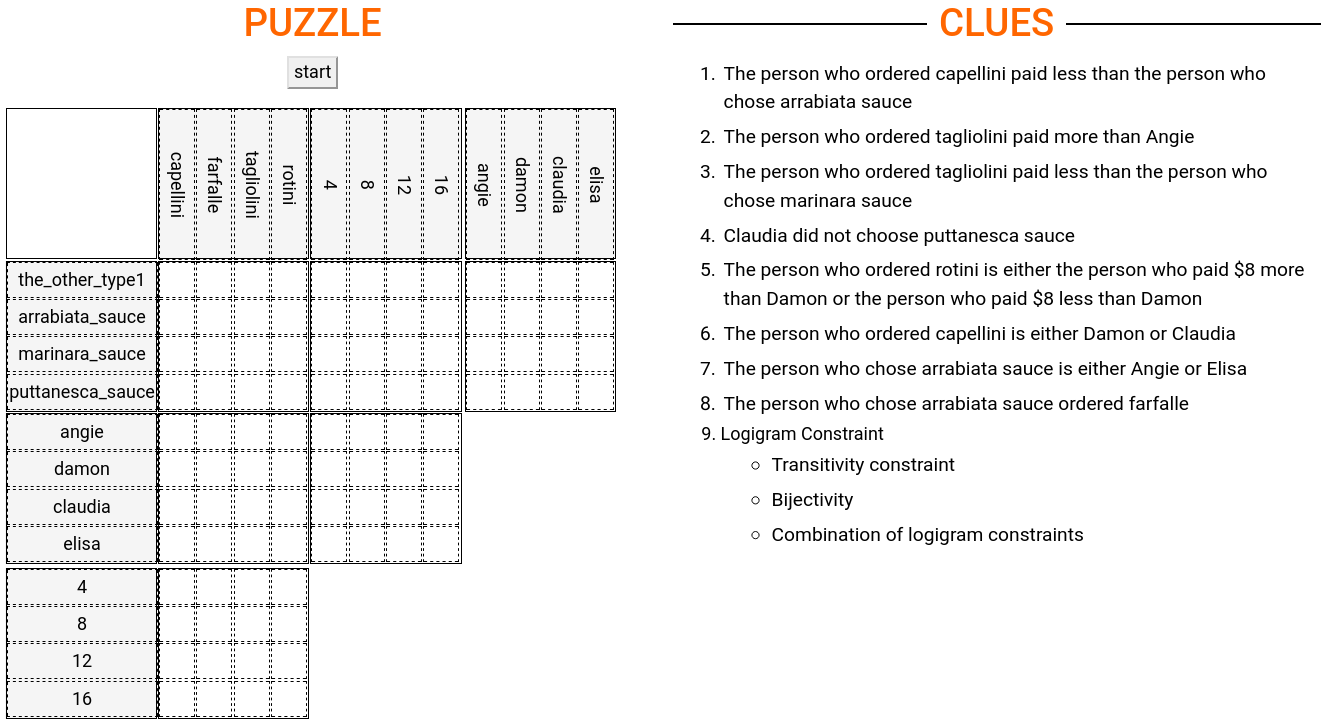
\includegraphics[width=\textwidth]{logicpuzzles.png}
	\end{figure}
\end{frame}

\begin{frame}{Motivation}
	\framesubtitle{Formalising CSPs}
	
\end{frame}




\begin{frame}{Motivation}
	\framesubtitle{Gentle reminder: Explanations for CSPs}
	 \begin{definition}
		Let $I_{i-1}$ and $I_i$ be partial interpretations such that $I_{i-1}\wedge T \models I_i$.
		We say that $(E_i,S_i,N_i)$ \emph{explains} the derivation of $I_{i}$ from $I_{i-1}$ if the following hold:
		\begin{itemize}
			\item $N_i= I_i \setminus I_{i-1}$ (i.e., $N_i$ consists of all newly defined facts), 
			\item $E_i\subseteq I_i$ (i.e., the explaining facts are a subset of what was previously derived),
			\item $S_i \subseteq T_P$ (i.e., a subset of the clues and implicit constraints are used), and 
			\item $S_i \cup E_i \models N_i$ (i.e., all newly derived information indeed follows from this explanation).
		\end{itemize}
	\end{definition}
\end{frame}

\begin{frame}{Motivation}
	\framesubtitle{Generating an explanation sequence for CSPs}
	
\end{frame}

\begin{frame}{Motivation}
	\framesubtitle{Open Questions}

   \begin{description}[font=\color{vuborange}\itshape]
	\item[\hspace{0.9cm}Optimality] Explanations not optimal, heuristically found
	\item[\hspace{1.05cm}Efficiency] Explanation generation takes a lot of time
	\item[\hspace{0.3cm}Incrementality] Can we reuse information from an explanation call to another?
	\item[Constrainedness] Can we avoid looping over the literals when searching for the next best explanation ?
   \end{description}
\end{frame}

\begin{frame}{Outline}

\end{frame}

\begin{frame}{Contributions}
    \vfill
    In this paper, we 
    \vfill
    \begin{itemize}
        \item ... introduce (cost-)\textbf{\underline{O}ptimal} \underline{U}nsatisfiable \underline{S}ubsets (OUS) using the minimal hitting set duality
        \item ... analyze the structural constraints of the OUS explanations
        \item ... improve the efficiency of explanation sequence generation
    \end{itemize}
    \vfill
\end{frame}

\begin{frame}{Use cases}
    \begin{itemize}
        \item Teach humans how to solve a certain problem
        \item Quantify problem difficulty
        \item ``Help'' button
        \item Interactive configuration/planning/scheduling
    \end{itemize}
\end{frame}

\begin{frame}{Conclusion and Future work}

\end{frame}

\begin{frame}[allowframebreaks]
	\frametitle{References}
	\bibliographystyle{named}
	\bibliography{references}
\end{frame}



\end{document}



